\section{Heartbeat Arrhythmia}
\begin{frame}{Heartbeat Arrhythmia}
    \begin{figure}
        \centering
        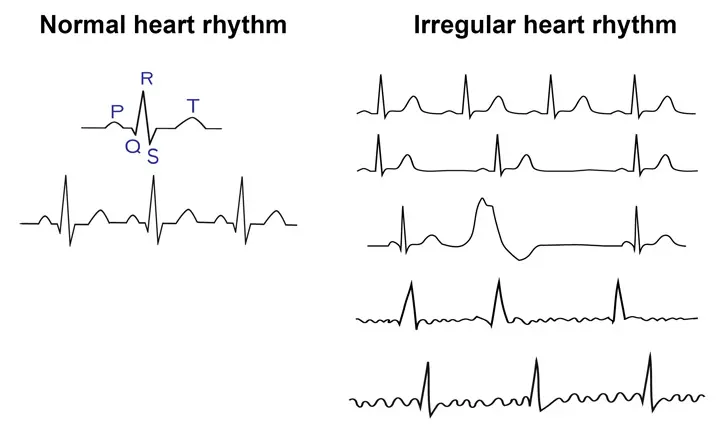
\includegraphics[scale=0.3]{images/heartbeat_arr.png}
        \caption[]{Different heartbeat arrhythmias \footnote{source: https://www.parkwayshenton.com.sg/health-plus/article/arrhythmia-guide}}
        \label{fig:enter-label}
    \end{figure}
\end{frame}

\begin{frame}{Arrhythmia Detection as an Anomaly Detection Problem}
We treat the problem of detecting irregular heartbeats as an anomaly detection problem from machine learning based on the reconstruction error:
\begin{itemize}
    \item We train a model on regular heartbeats that is able to reconstruct that regular heartbeat.
    \item Given an irregular heartbeat the model should give higher reconstruction error.
    \item Based on an optimal threshold for that error we classify this heartbeat as either regular or irregular.
\end{itemize}
    Two reasons for this semi-supervised approach: high class imbalancy and no need for labelling.
\end{frame} 

\begin{frame}{Baseline Model}
    Model is a LSTM-AE that is trained only on normal samples with the goal to reconstruct normal samples. The classification is made based on the reconstruction error.
    \begin{columns}
        \begin{column}{0.48\textwidth}
        \begin{figure}
            \centering
            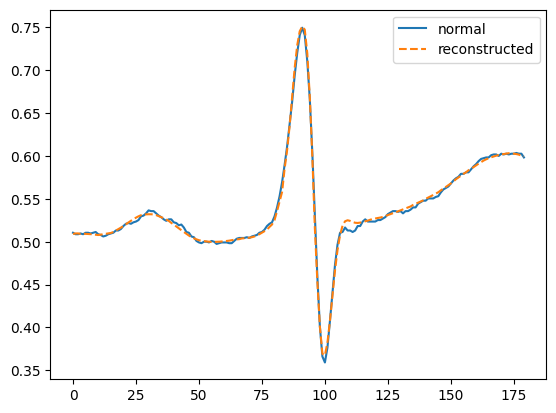
\includegraphics[scale=0.3]{images/rec_normal.png}
            \caption{reconstruction on normal sample \phantom{asdfsadf}}
            \label{fig:enter-label}
        \end{figure}
    \end{column}
    \begin{column}{0.48\textwidth}
        \begin{figure}
            \centering
            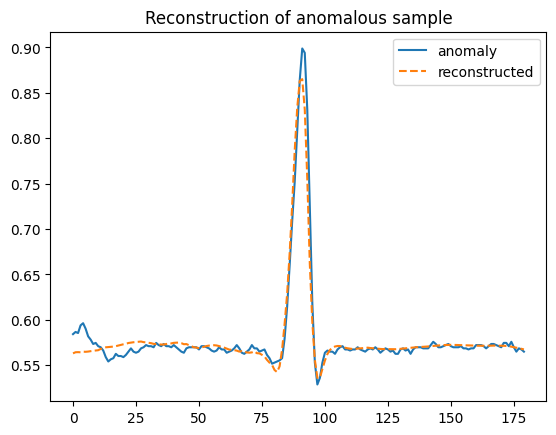
\includegraphics[scale=0.3]{images/rec_anom.png}
            \caption{reconstruction on anomalous sample}
            \label{fig:enter-label}
        \end{figure}
    \end{column}
    \end{columns}
\end{frame}